
\chapter{FUNDAMENTAÇÃO TEÓRICA}
\label{c.fundamentacao}

Neste capítulo é apresentado o plano de fundo teórico que envolve os tópicos
pertinentes ao trabalho, destacando as definições e conceitos essenciais dos
seguintes assuntos: Redes de Computadores, Internet, Segurança em redes de
Computadores (estado da arte), \textit{Malware} e suas respectivas técnicas de
detecção.
\section{Redes de Computadores e Internet}
\label{s.teoria_redes_internet}

Segundo o trabalho de KUROSE (\citeyear{kurose09}), pode-se definir a Internet
como a rede de computadores que interconecta milhões de dispositivos
computacionais ao redor do mundo. Há pouco tempo a gama de dispositivos
conectados à internet era mais baixa e se resumia a servidores e computadores
de mesa. Hoje pode-se ver que cada vez mais dispositivos não tradicionais
estão sendo ligados à internet. Assim, define-se como sistemas finais, ou
hospedeiros, quaisquer dispositivos que possuam tal capacidade de conexão. Em
julho de 2008 estimavam-se 600 milhões de sistemas finais ligados à internet
sem contar dispositivos que são conectados de maneira intermitente (como
laptops e smartphones). Quando sistemas finais se comunicam, trocam arquivos
segmentados, que denominam-se como pacotes, por meio de enlaces de comunicação
(\textit{links}), que podem ser físicos ou por ondas, no caso de redes sem fio e via
rádio. Os dispositivos periféricos que são responsáveis por essa comunicação
são chamados comutadores de pacotes, vistos comumente como roteadores e
\textit{switchs}. O que torna essa comunicação válida entre tantos dispositivos
diversos são os protocolos de rede, como TCP/IP. Tais protocolos apenas
definem a estrutura dos pacotes que serão trocados e a classificação dos dados
dentro destas estruturas. Dessa maneira, os comutadores de pacotes conseguem
interagir sem problemas e dividir as cargas da rede com eficiência. Neste
trabalho não se faz necessária uma abordagem mais profunda sobre estruturas de
pacotes e de componentes mais específicos da rede, haja visto que o foco do
trabalho é voltado para segurança em redes e uma revisão completa sobre
fundamentos básicos de redes não elucida conteúdos dessa vertente. Os pacotes
ainda serão citados no decorrer do trabalho e terão seus conceitos devidamente
esclarecidos na seção apropriada. A ideia geral de redes de computadores
suficiente para esse trabalho pode ser ilustrada com a figura 2:

\begin{figure}[H]
\caption{\small Alguns componentes da internet}
\centering
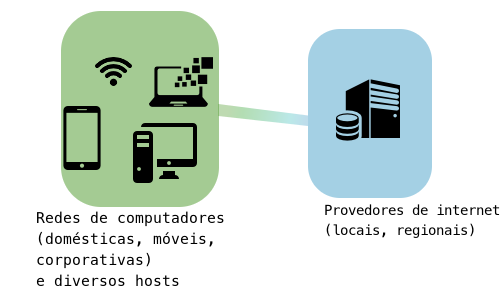
\includegraphics[scale=0.5]{figs/fig3_teste.png}
\label{f.internet_01}
\legend{\small Fonte: Kurose (2009) (adaptada pelo autor)}
\end{figure}

\section{Segurança em redes de computadores}
\label{s.seguranca}

Para KUROSE (\citeyear{kurose09}), pode-se definir vários conceitos em segurança de
redes. A ideia em si vem de imaginar que as pessoas desejam se falar através da
internet, por exemplo, e que essas pessoas não queiram que ninguém mais seja
capaz de interceptar esses dados mesmo que elas estejam conectadas em locais
considerados inseguros, que deixam computadores serem publicamente utilizados.
Além disso, imaginar que as pessoas também querem garantir que as mensagens
trocadas não sejam originadas de um intruso, ou passem por um intruso na rede.
Com essa ideia somos capazes de elencar as propriedades necessárias para uma
comunicação considerada \emph{segura}. São elas:

\begin{itemize}
\item[-] Confidencialidade: A garantia de que somente respectivos remetentes e destinatários sejam capazes de ver e entender o conteúdo das mensagens transmitidas.
\item[-] Autenticação do ponto final: Remetentes e destinatários precisam ter meios de confirmar a identidade uns dos outros durante uma comunicação.
\item[-] Integridade da mensagem: Além de identificarem uns aos outros, os envolvidos na comunicação querem assegurar que o conteúdo que enviem seja exatamente o conteúdo que as outras partes recebam. As mensagens podem se corromper durante uma comunicação tanto por acidentes, como por má intenção de intrusos na rede.
\item[-] Segurança Operacional: Qualquer empresa atualmente vai ter uma rede local conectada à rede pública. Os mecanismos responsáveis por filtrar o que a rede local vai receber da rede pública são chamados mecanismos de segurança operacional, como \textit{firewalls}, que são servidores que se posicionam entre as duas redes e intermedeiam a comunicação entre elas, e também como sistemas de detecção de intrusão, foco maior do trabalho, que são sistemas que analisam os pacotes de maneira mais profunda e os identificam para separar e tratar pacotes potencialmente suspeitos.
\end{itemize}

Qualquer ação de um intruso na rede configura uma falha na presença de um ou
mais dos quesitos elencados acima; quando ocorre tal brecha e um usuário
estranho consegue acesso não autorizado a uma rede, ele ganha muitas
possibilidades de uso para essa rede. Um invasor pode agir de modo passivo
apenas monitorando as comunicações que pode ver, ou então agir com um caráter
mais nocivo e alterar os conteúdos que acessa, seja corrompendo, alterando ou
removendo arquivos, senhas e dados diversos. Os sistemas de detecção de
intrusão buscam maneiras de identificar acessos ilegais e tráfego de dados
estranhos na rede. \subsection{Estado atual da área de segurança de redes}
\label{sub:estado_da_arte}

De acordo com Hurd (\citeyear{hurd15}) uma área bastante promissora é a de
\emph{Cyber Higiene}, e seus aspectos incluem gerenciamento e proteção de credenciais,
auditoria de roubo de credenciais e dados analíticos sobre comportamento de
acesso do usuário, sendo esta última subárea a que demonstra a maior parcela
de progresso recente e num futuro de médio prazo. Nesse segmento, o conceito
de usuário pode ser especificado além do usuário comum, classificando novos
perfis como atacantes e autores (programadores). O comportamento envolve
características como duração do tempo de acesso, preferência de dispositivo
utilizado, utilização de navegador e outras diversas informações sobre as
atividades desenvolvidas por um usuário e quais seriam seus fins. Utilizando a
internet como ``observatório'' , a análise do comportamento de
usuários tem sofrido uma revolução em virtude do crescimento da internet das
coisas, onde cada vez mais objetos estão conectados à rede, com grande parte
destes objetos sempre reportando informações, como sensores e câmeras de
trânsito.


\section{Malware}
\label{s.malware_01}

O conceito de \textit{Malware} já foi abordado de maneira mais rudimentar na introdução
do trabalho. Porém, como o viés do projeto caminha muito próximo de
classificações mais profundas desse tópico, faz-se necessário recorrer a uma bibliografia mais
completa sobre os processos relacionados ao \textit{Malware}. Na pesquisa desenvolvida
por SAHEED(\citeyear{saeed13}), pode-se aproveitar muitas informações sobre o
patamar do desenvolvimento deste tipo de \textit{software}. De acordo com pesquisas
levantadas pela McAfee\footnote{www.mcafee.com}, esses programas continuam a se tornar mais numerosos
dia-a-dia, sendo encontrados novos ``indivíduos'' aos milhares. Em
contrapartida, pesquisadores e laboratórios especializados em segurança
aprimoram novos métodos para construir \textit{anti-malware} mais eficiente e mais
autônomo. A seguir, diferenciam-se os tipos de \textit{Malware} com base nas técnicas de
criação dos mesmos, separando-os por técnicas de ofuscamento, métodos de
invocação, plataforma de atividade, abrangência e técnicas de propagação. Nem
todo \textit{software} malicioso é executado de dentro de máquinas infectadas;
atualmente a maioria dos ataques são originários da internet, pois as
vulnerabilidades encontradas são mais proeminentes do que em ambientes de rede
local, em virtude de a internet ser um espaço, de modo geral, público,
beneficiando atacantes que tenham meios de acessar um sistema alvo
remotamente. Um sistema de detecção de \textit{malware} tem majoritariamente duas
tarefas: busca e análise, ou seja, saber encontrar material não confiável e
saber identificar com precisão que o material em questão realmente possui
traços nocivos de código, ou faz com que algum outro programa apresente
comportamento considerado anormal.

\subsection{Técnicas de criação}
\label{ss.tecnicas}

Para criar esse tipo de código, atacantes utilizam de vários meios desde a
inserção de pequenos pedaços de código em outros programas, até a algoritmos
de alta complexidade, feitos com o intuito de esconder o \textit{malware} ou torná-lo
\emph{polimórfico}. Um \textit{malware} que se classifique como polimórfico consiste em
um programa capaz de trocar pedaços do código sem mudar a semântica e o
resultado da execução a cada infecção, para driblar verificações de sintaxe,
geralmente com a ajuda de técnicas avançadas de encriptação. \textit{Malwares}
polimórficos são o grande ponto fraco das técnicas de detecção por assinatura,
pois eles tornam inviável a geração de assinaturas únicas para classificação
do código malicioso. Pode-se dizer que um \textit{Malware} é \emph{ofuscado} quando ele é
polimórfico ou \emph{metamórfico}, onde o código original é transformado em
algo funcionalmente equivalente, porém muito mais difícil de se compreender
quando lido. As técnicas utilizadas para que isso ocorra são a utilização de
código morto, que é uma grande parcela de código que não faz absolutamente
nada, acoplado ao código malicioso para mascará-lo, ou também a transportação
de código, que consiste em realizar um grande número de ``jumps'' no programa,
porém sem alteração no fluxo de controle do mesmo.

\subsection{Malware baseado em rede}
\label{ss.malware_rede}

Para dar início à classificação dos tipos de \textit{Malware}, primeiro observa-se com
destaque aqueles que se utilizam da rede como meio de propagação e de atuação.
Nesse segmento, é possível identificar o que são os \textit{Adwares}, \textit{Spywares}, \textit{Cookies},
\textit{Backdoors}, \textit{Trojans}, \textit{Sniffers}, \textit{Spam} e \textit{Botnet}.

\textit{Spyware} é um tipo de \textit{malware} que se instala de maneira secreta num computador,
com o objetivo de coletar informações sobre o uso de determinados programas ou
sites visitados por um indivíduo sem o conhecimento do mesmo. Curiosamente,
até mesmo grandes empresas como Google e Microsoft se utilizam desse tipo de
\textit{Malware} para coletar informações de seus clientes.

\textit{Adwares} são feitos com a finalidade de servirem como atalhos publicitários
para outros programas que têm seu desenvolvimento mantido com fundos oriundos
de propaganda na internet. Por natureza, não são essencialmente danosos a
sistemas e no máximo causam transtorno às pessoas por apresentarem anúncios
indesejados, entretanto, existem algumas variações nessa família de \textit{malware}
que possuem \textit{spyware} acoplados juntamente com as propagandas, invadindo a
privacidade dos usuários.

\textit{Cookies}, na verdade, são informações de usuário guardadas pelos navegadores de
internet; eles servem primeiramente como meio de autenticação e armazenamento
de configurações entre cliente e servidor. Um cookie é um pequeno arquivo de
texto com essas informações, e na maioria das vezes vai ter um prazo de
validade fixado pelo servidor que o usuário acessa. Também não são danosos,
mas os \textit{cookies} são usados por \textit{spywares} e também no roubo de credenciais de
usuários.

\textit{Backdoors} ou \textit{Trapdoors} são código malicioso atrelado a aplicações ou sistemas
operacionais que concedem a alguém acesso a um sistema sem que seja necessário
passar por métodos comuns de autenticação. Eventualmente esses programas
também podem ser usados como meio para conseguir acesso remoto a sistemas.

Um \textit{Trojan Horse} (cavalo de tróia), ou apenas \textit{Trojan}, descreve um programa que
aparenta ser útil ou inofensivo, mas que ao ser executado pode corromper dados
ou roubar informações. Um \textit{Trojan} é desenvolvido para que o usuário, além de
não suspeitar dele, seja levado a executá-lo por curiosidade, então é muito
comum ver esse tipo de programa escondido em arquivos multimídia que vão
seduzir algum nicho de usuários.

\textit{Sniffers} são capazes de monitorar e armezenar dados a respeito do tráfego de
uma rede. Eles capturam os pacotes que estão sendo trocados e os decodificam
para ganhar acesso aos dados crus dos campos dos pacotes. \textit{Sniffers} podem ser
usados como um passo inicial para uma invasão, para que posteriormente sejam
obtidas senhas e outras informações confidenciais que sejam alvo de um
atacante.

O \textit{Spam} talvez seja o tipo de \textit{malware} mais conhecido por usuários mais leigos;
basicamente é um pacote de \textit{software} com a funcionalidade de transmitir
mensagens em larga escala via \textit{e-mail}. O impacto negativo do \textit{spam} é a
possibilidade de lentidão causada pelo alto número de requisições que será
realizado por ele para os servidores, atrapalhando o recebimento de mensagens
mais relevantes e poluindo as caixas de \textit{e-mail}. Embora seja uma prática muito
mal vista na internet, nos Estados Unidos o \textit{spam} é legalizado, graças ao ato
CAN-SPAM, desde 2003.

\textit{Botnet} não é na verdade um \textit{malware} de código, mas uma coleção de computadores
infectados e que são controlados remotamente por um atacante que pode usá-los
para realizar atos maldosos sem que seja preciso se autenticar nessas
máquinas. Esse é o conceito por trás dos ataques de negação de serviço (DoS),
onde um grande número de máquinas controladas sobrecarrega um determinado
serviço na rede com um número absurdo de requisições aos servidores.(SAHEED, 2013)

\subsection{Malware Comum}
\label{ss.malware_comum}

O \textit{Malware} comum, em contraste com o de rede, é feito para ser executado em
ambiente local sem a necessidade de qualquer conexão a rede, pois também pode
ser propagado via dispositivos físicos como pendrives, HDs externos e
periféricos com \textit{software} malicioso embarcado. Nessa categoria, classificam-se os vírus, \textit{worms} e bombas lógicas.

Vírus de computador é um conceito que muitas vezes acaba generalizando o
\textit{Malware}. É muito comum um usuário que foi infectado apenas com \textit{adware} dizer
que ``está com vírus no PC'' e assim segue; Na verdade, um vírus de computador
é um código capaz de se replicar durante a infecção em qualquer programa ou
documento. Por exemplo, sistemas Windows em muitas mídias se utilizam de um
arquivo ``autorun.inf'' para automatizar a execução de tarefas para montagem
de pastas ou imagens de disco. Logo, um código maldoso que possa se acoplar
silenciosamente a esse tipo de arquivo, com certeza conseguirá infectar um
sistema Windows.

Os \textit{Worms} são códigos capazes de se replicar em múltiplas máquinas de modo
independente, isto é, sem precisar se atrelarem a um determinado programa para
iniciar seu ciclo de vida. Eles podem, entre outras coisas, consumir a banda
da rede e privar o usuário infectado de utilizá-la, além de criarem várias
cópias de si para aumentar a taxa de programação. Esta última característica é
o que os \textit{softwares} de anti-vírus utilizam para identificar \textit{Worms}; se um
arquivo está se repetindo muitas vezes com atributos iguais, ele é considerado
suspeito nesses sistemas de detecção.

A bomba lógica é um \textit{software} que permanece quieto até que se atinja uma
determinada condição. Para isso, o programa fica apenas checando a data do
sistema até que seja a data especificada e só então ele vai, de fato, executar
seu código.(SAHEED, 2013)

Dadas essas classificações, pode-se ilustrar os tipos de \textit{malware} e suas características com o quadro 1:
\renewcommand{\thequadro}{\arabic{quadro}}

\begin{quadro}[H]
\caption{\small Famílias de \textit{Malware} e fatores comparativos}
\centering
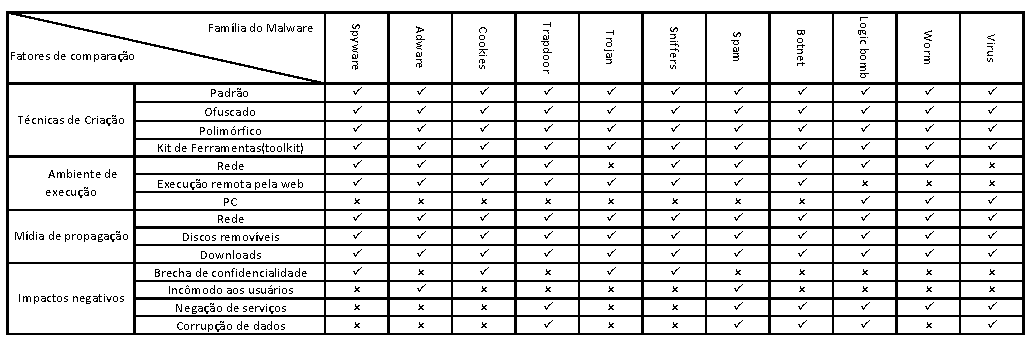
\includegraphics{figs/tabela.pdf}
\label{f.tabelamalware}
\legend{\small Fonte: Saeed (2013) (traduzida pelo autor).}
\end{quadro}

\subsection{Código fonte de Malware} % (fold)
\label{ssub:exemplos_malware}

Alguns \textit{malwares} acabam tendo seu código aberto e disponibilizado para
estudos, ora por vontade de seus próprios autores, ou por vazamento de
informações feito por outros \textit{hackers} interessados em tornar público
esse tipo de informação. A cada ano, o nível de complexidade para a construção
de \textit{malwares} fica maior, pois como a maior parte deles é voltada para
ataques em rede, é preciso pensar numa aplicação funcional com arquitetura do
tipo cliente-servidor, contendo além de todos os algoritmos que explorem
vulnerabilidades, os meios de encriptação e disfarce do \textit{malware}. Ou
seja, até mesmo o menor dos \textit{malwares} construídos hoje em dia, possui
muito código embutido e embaralhado dentro de si, a fim de dificultar o processo
de detecção e mapeamento de assinaturas.

\section{Detecção}
\label{s.deteccao}

Nesta seção, é exposto o estado atual das tecnologias de
detecção e para onde elas estão caminhando no futuro. O trabalho de
Baddar et al. (\citeyear{baddarxx}) nos mostra uma perspectiva bastante atual do cenário e
de como funcionam, de modo geral, os processos de detecção das anomalias. Um
sistema de detecção pode agir em ambiente de rede, verificando as
características do tráfego da rede, ou em nível de aplicação, onde vai varrer
os dados do disco a procura de assinaturas conhecidas de anomalia ou de
comportamentos fora do normal. A detecção por comportamento anômalo precisa
ser capaz de filtrar casos anômalos isolados, denominados como anomalias
pontuais, de casos com suspeita mais palpável de anomalia, que pode-se chamar de
anomalia de contexto. Uma anomalia pontual pode ser exemplificada do seguinte
modo: uma tentativa de acesso de um usuário num sistema corporativo não é, a
princípio, um ato que possa ser classificado como anômalo; porém, se essa
mesma tentativa se repete várias vezes em horários não condizentes com o
expediente comercial, pode haver alguém suspeito tentando roubar as
credenciais desse usuário. As figuras 3 e 4 exemplificam as ideias de
anomalia pontual e contextual:

\begin{figure}[H]
\caption{\small Exemplo de anomalia pontual}
\centering
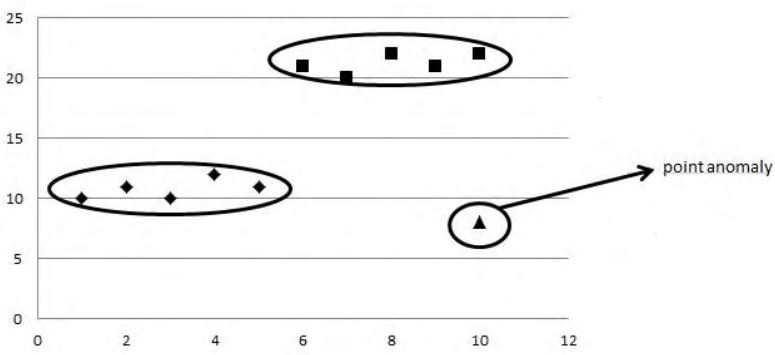
\includegraphics[scale=0.6]{figs/anomalia_pontual.JPG}
\label{f.anomalia_pontual}
\legend{\small Fonte: Baddar. (\citeyear{baddarxx})}
\end{figure}

\begin{figure}[H]
\caption{\small Exemplo de anomalia contextual}
\centering
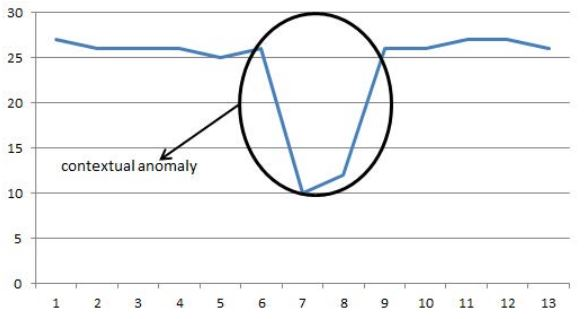
\includegraphics[scale=0.6]{figs/anomalia_contextual.JPG}
\label{f.contextual}
\legend{\small Fonte: Baddar. (\citeyear{baddarxx})}
\end{figure}

\subsection{Detecção baseada em funcionalidade}
\label{ss.deteccao_funcionalidade} Destaca-se esse segmento em especial pois é
daqui que se origina a ideia de detecção baseada em assinaturas e em
comportamentos. A detecção baseada em assinaturas compara casos suspeitos com
uma relação já conhecida de código comprovadamente nocivo, que fica armazenada
geralmente num banco de dados da empresa que desenvolve o sistema de detecção.
Motores de busca de anti-vírus são o exemplo mais clássico de detecção baseada
em assinaturas. Numa outra abordagem, a detecção por comportamento vai tentar
``aprender'' como vive um programa normal dentro do sistema, e como é o ciclo
de um programa suspeito, geralmente recorrendo a dados de tempo de execução
dos programas que estão sendo processados e classificando essas
características com o auxílio de técnicas como aprendizado de máquina e redes
neurais (BADDAR, \citeyear{baddarxx}). A maior parte do conjunto recente das aplicações de detecção
em nível de rede tem adotado a abordagem do aprendizado de máquinas para
detectar \textit{software} por comportamento, quando em nível de rede. Em nível de
aplicação, a grande maioria também procura traçar perfis de comportamento
utilizando técnicas de detecção em modo dinâmico como pode-se ver nos quadros
2 e 3, a seguir:

\begin{quadro}[h]
\caption{\small Tecnologias recentes de detecção em nível de rede}
\centering
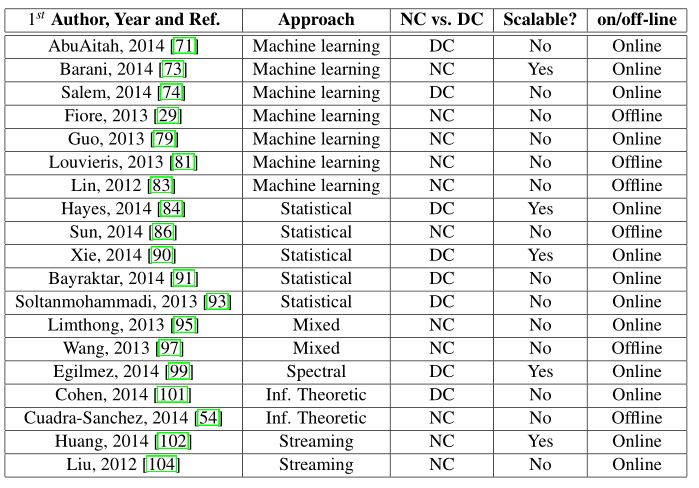
\includegraphics[scale=0.6]{figs/tabela_deteccao_nivel_rede.JPG}
\label{f.tabeladeteccao_rede}
\legend{\small Fonte: Baddar. (\citeyear{baddarxx})}
\end{quadro}

\begin{quadro}[h]
\caption{\small Tecnologias recentes de detecção em nível de aplicação}
\centering
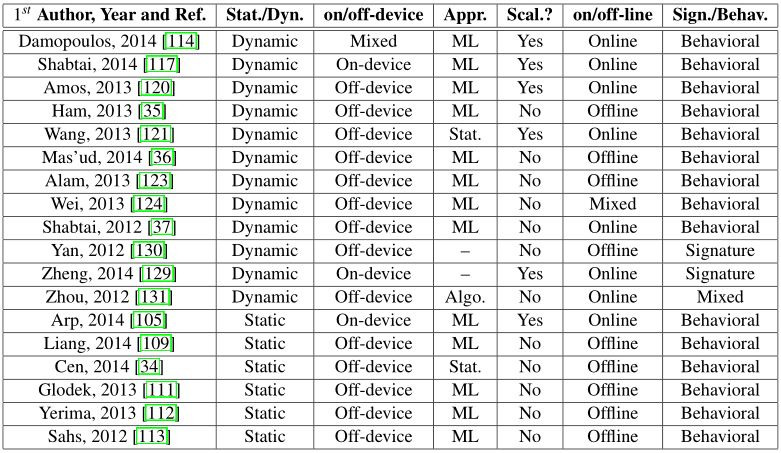
\includegraphics[scale=0.6]{figs/tabela_deteccao_nivel_aplicacao.JPG}
\label{f.tabeladeteccao_app}
\legend{\small Fonte: Baddar. (\citeyear{baddarxx})}
\end{quadro}
